\begin{homeworkProblem}[Quiz 4]
    \textbf{Two charges are separated by a distance of 2a. One charge,
    $q_1 = +q$ and the other charge $q_2 = -q$. Find the potential due
    to these charges a very far distance from the two charges. To solve
    for this potential, express the potential everywhere in space as the
    sum of the potentials generated by each point charge. Then, perform
    a 1st order expansion of the potential.}
    \\

    \begin{figure}[t]
        \centering
        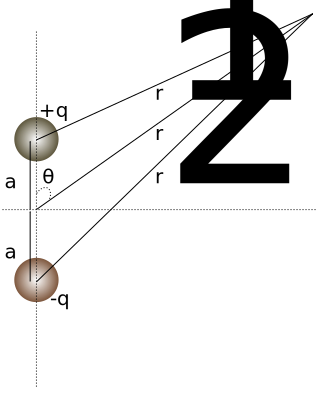
\includegraphics[width=.45\textwidth]{./img/charges.pdf}
        \caption{Diagram of Quiz Problem \#4}
        \label{fig:charges.pdf}
    \end{figure}

    Okay, the instructions tell us what to do at the very beginning. Our
    first goal will be to express the potential everywhere in space. We
    know that the potential $V(\vec{r})$ at a point $\vec{r}$ due to a
    point charge $V(\vec{r}) = \frac{k q}{r} $. Now, that $r$ in the
    denominator is the distance that I am away from the point charge.
    So, for a point charge not located at the origin, I should really
    express this as $V(\vec{r}) = \frac{kq}{|\vec{r}-\vec{r}'|}$. See
    Fig.~\ref{fig:charges.pdf} for a diagram that explains this relationship.
    For this problem, then, the potential at a point $\vec{r}$ is

    \[
    V(\vec{r}) = \frac{k q_1}{r_1} + \frac{k q_2}{r_2}
    \]

    Now, $\vec{r_2}=\vec{a}+\vec{r}$ and $\vec{r_1}=\vec{r}-\vec{a}$.
    Here $a$ is the vector that points from the negative charge to the
    origin. It is also the negative of the vector that points from the
    positive charge to the origin. Thus, $|\vec{r_2}|=|\vec{a}+\vec{r}|$
    and $|\vec{r_1}| = |\vec{r}-\vec{a}|$. It would be nice if we could
    get rid of these absolute value signs. We really want to know how
    big $\vec{r_2}$ is and how big $\vec{r_1}$ is. For that, we'll
    employ the following identity: $|\vec{v}|=
    \sqrt{\vec{v}\cdot\vec{v}}$. You can justify this by realizing that
    $\vec{a}\cdot\vec{b}=|\vec{a}|.  |\vec{b}|\cos\theta$.

    \[
    V(\vec{r}) = \frac{k
    q_1}{\sqrt{\vec{r}\cdot\vec{r}+\vec{a}\cdot\vec{a}-2|\vec{a}||\vec{r}|\cos\theta}}
    + \frac{k
    q_2}{\sqrt{\vec{r}\cdot\vec{r}+\vec{a}\cdot\vec{a}+2|\vec{a}||\vec{r}|\cos\theta}}
    \]

    But, $\vec{r}\cdot\vec{r}$ is simply $|\vec{r}|^2 = r^2$.
    Also,$\vec{a}\cdot\vec{a}$ is simply $|\vec{a}|^2 = a^2$. Thus,

    \[
    V(\vec{r}) = \frac{k q}{\sqrt{r^2+a^2-2ar\cos\theta}} + \frac{k
    q}{\sqrt{r^2+a^2+2ar\cos\theta}}
    \]
   
    Note that I have also inserted the signs of the two charges in the
    last line. Now, the problem asks us to solve for the potential when
    $r \gg a$. Thus, I will factor out an $r$ from the previous
    expression's denominator to express everything in terms of the
    ratio $\frac{a}{r}$.

    \begin{align}
        \label{}
        V(\vec{r}) &=  \frac{k q}{r} \left( 
        \frac{1}{\sqrt{1+\left( \frac{a}{r} \right)^2-2\left(
        \frac{a}{r} \right)\cos\theta}}
        -\frac{1}{\sqrt{1+\left( \frac{a}{r} \right)^2+2\left(
        \frac{a}{r} \right)\cos\theta}}
        \right) \nonumber \\
        &= \frac{k q}{r} 
        \left(
        \frac{1}{\sqrt{1+\epsilon^2-2\ \epsilon \cos\theta}} -
        \frac{1}{\sqrt{1+ \epsilon^2+2 \epsilon \cos\theta}}
        \right) \nonumber
    \end{align}

    Here, I have replaced the quantity $\frac{a}{r}$ with the small
    quantity $\epsilon$. This is nothing more than simple variable
    substitution. Now, I realize that I can expand this function about
    small $\epsilon$ and I would be done. However, expanding about
    $\epsilon$ would make my life a litle difficult because I would have
    to take derivatives of $V(\epsilon)$ with respect to $\epsilon$ which
    would involve using the chain rule to evaluate the derivative of
    $(1+\epsilon^2\pm2\epsilon\cos\theta)^{-.5}$. Okay, at this point, I
    have two ways that I can solve the problem so I will diverge and I
    will show you the preferred way, first (this is the way that I
    requested you all do it). I recommend you read both approaches.

    \begin{homeworkSection}{Expanding Around $f$}

    I'm going to do a little trick that makes my life a lot easier. Note
    that $\epsilon^2 \pm 2\epsilon\cos\theta$ is just a function of
    $\epsilon$. I could just wrap this whole expression up inside
    something else. Let's call $f^+(\epsilon) \equiv \epsilon^2 + 2
    \epsilon\cos\theta$ and $f^-(\epsilon) \equiv
    \epsilon^2-2\epsilon\cos\theta$ (triple horizontal bars mark a
    definition).
    
    Note that as $\epsilon \rightarrow 0$, $f^\pm(\epsilon) \rightarrow
    0$. Thus, expanding about small $\epsilon$ is the same as expanding
    around small $f$. So, for any value of $r$ we are considering
    (assuming, still, that $r \gg a$) we can expand $V(f^+,f^-)$ around
    small
    $f^+$ and $f^-$. Our expression for $V(f^+,f^-)$, now, is:

    \begin{align}
        \label{}
        V(\vec{r}) &= \frac{k q}{r} \left(
        \frac{1}{\sqrt{1+f^{-}(\epsilon)}} - 
        \frac{1}{\sqrt{1+ f^{+}(\epsilon)}}
        \right) \nonumber \\
        &= \frac{k q}{r} \left(
        \left[ 1+f^{-}(\epsilon)  \right] ^{-.5} - 
        \left[ (1+ f^{+}(\epsilon)  \right]^{-.5}
        \right) 
    \end{align}

    Now, I will introduce the math necessary to perform a Maclaurin
    series expansion of $V(\vec{R})$. A Maclaurin series expansion of a
    function $g(x)$ is the Taylor series expansion of $g$ about $x=0$
    (yeah, that gets a special name). Just remember that a Maclaurin
    series is a Taylor series of a function centered about zero. The
    Taylor series of a function $g(x)$ about the point $x = a$,
    $T(g(x))|_{x=a}$ is defined as:

    \[
    T(g(x))|_{x=a} = \sum\limits_{n=0}^{\infty}\frac{g^{n}(a) (x-a)^n}{n!}
    \]

    Here, I have used the notation $g^{n}(a)$ as a succinct form of
    $\frac{\diff^n g(x)}{\diff x^n}|_{x=a}$. For a Maclaurin series (one
    where $a=0$) this can be reduced to:

    \[
    T(g(x))_{x=a} = \sum\limits_{n=0}^{\infty}\frac{g^{n}(0) x^n}{n!}
    \]

    The most significant reduction to this expression is in the
    $(x-a)^n$ term. We have only been asked to expand the potential to
    first order. But, for demonstrative purposes, let's expand to 2nd
    order. At this point you should be asking the question: ``How do I
    expand $V(f^+,f^-)$? There are two variables: $f^+$ and $f^-$''. The
    way in which we're going to get around this is by expanding two
    other functions $g^+ = (1+f^+)^{-.5}$ and $g^- = (1+f^-)^{-.5}$ to
    second order in $f^+$ and $f^-$, respectively. Then, we'll combine
    the expressions to solve for $V$. An approximate expression for
    $V(\vec{r})$ then, to second order is:
    
    \begin{align}
        \label{}
        V &= \frac{k q }{r} \left( g^-(f^-) - g^+(f^+) \right) \nonumber
        \\
        V &\approx \frac{k q }{r} \left( 
        \left( {g^-}^0(0) + {g^-}^1(0) f^- + \frac{{g^-}^2(0)
        {f^-}^2}{2} \right)-
         \left( {g^+}^0(0) + {g^+}^1(0) f^+ + \frac{{g^+}^2(0)
        {f^+}^2}{2}  \right)
        \right)
        \nonumber
   \end{align}
   
    Okay, that looks pretty complicated, but it's not. The first three
    terms in parentheses are just the 0 to 2nd order terms of the
    Maclaurin series expansions of $g^+ = (1+f^+)^{-.5}$ and the second
    three terms are just the 0 to 2nd order terms of $g^- =
    (1+f^-)^{-.5}$ - Don't forget that I'm using the shorthand $f^n(a) =
    \frac{d^n f(x)}{dx^n}|_{x=a}$. One thing that simplifies the
    previous expression a lot is the fact that $g^+(0) = g^-(0) = 1$. I
    will substitute this expression in and, in the following lines, I
    will take the 1st and second derivatives of $g^+$ and $g^-$ and I'll
    evaluate ${g^\pm}^1(0)$ and ${g^\pm}^2(0)$.
    \begin{align}
        \label{}
        V &\approx \frac{k q }{r} \left( 
        \left( 1 + {g^-}^1(0) f^- + \frac{{g^-}^2(0)
        {f^-}^2}{2} \right)-
        \left( 1 + {g^+}^1(0) f^+ + \frac{{g^+}^2(0)
        {f^+}^2}{2}  \right)
        \right) \nonumber
        \intertext{Now, evauluating ${g^+}^1(0)$:} \nonumber\\
        {g^+}^1(0) &= \frac{\diff}{\diff f^+} (1-f^+)^{-.5}|_{f^+=0}
        \nonumber \\
        &= -\frac{1}{2} (1-f^+(0))^{-\frac{3}{2}} \nonumber \\
        &= -\frac{1}{2} \nonumber \\
        \intertext{Remember that $f^+(0) = 0$. Now, evaluating
        ${g^+}^2(0)$:} \nonumber \\
        {g^+}^2(0) &= \frac{\diff^2}{\diff {f^+}^2} (1-f^+)^{-.5}|_{f^+=0}
        \nonumber \\
        &= -\frac{1}{2}\frac{\diff}{\diff f^+}
        (1-f^+)^{-\frac{3}{2}}|_{f^+=0} \nonumber \\
        &= \frac{3}{4} \left(1-f^+(0) \right)
        \nonumber \nonumber \\
        &= \frac{3}{4} \nonumber
    \end{align}
 
    Now, I only found the 2nd order derivative of $g^+(f^+)$. I have to
    do the whole thing again for $g^-(f^-)$. But, before I do that,
    realize that the only thing that would change if I did this would be
    that everywhere I had an $f^+$ in the previous expressions I would
    have an $f^-$, now. But $f^+(0) = f^-(0) = 0$ so my derivatives for
    $g^-$ would be the same as those for $g^+$. Thus, I can just recycle
    my results. Now, I can finally write my expression for $V\left(
    f^+(\epsilon),f^-(\epsilon) \right)$:

    \begin{align}
        \label{}
        V &\approx \frac{k q }{r} \left( 
        \left( 1 -\frac{1}{2} f^- + \frac{3}{4} 
        \frac{{f^-}^2}{2} \right)
        -
        \left( 1 - \frac{1}{2}f^+ + \frac{3}{4}
        \frac{{f^+}^2}{2}  \right)
        \right)
        \nonumber
    \end{align}

    Okay, notice that the two ``1s'' cancel. I can substitute my
    expressions for $f^+(\epsilon)$ and $f^-(\epsilon)$ into the
    previous expression:

    \begin{align}
        \label{}
        V &\approx \frac{k q }{r}
        \left(
            \left(
                -\frac{1}{2}
                \left( \epsilon^2 -2\epsilon\cos\theta
                \right)
                +\frac{3}{4}
                \frac{\left(\epsilon^2 -2\epsilon\cos\theta \right)^2}{2}
            \right)
            -\left( 
                -\frac{1}{2}(\epsilon^2 + 2\epsilon\cos\theta)+ \frac{3}{4}
                \frac{\left(\epsilon^2+2\epsilon\cos\theta \right)^2}{2}
            \right)
        \right) \nonumber \\
        V &\approx \frac{k q }{r}
        \left(
            -\frac{1}{2}\epsilon^2 + \epsilon\cos\theta+ \frac{3}{8}
            \left(
                \epsilon^2 - 2\epsilon\cos\theta
            \right)^2  
            +\frac{1}{2} \epsilon^2 +\epsilon\cos\theta -\frac{3}{8}
            \left(\epsilon^2 +2\epsilon\cos\theta
            \right)^2
        \right) \nonumber
    \end{align}

    Let's simplify this expression. Notice that the $\epsilon^2$ and
    $\epsilon^4$ terms from all the terms will go away (even the term
    that I have not explicitly squared, yet). Only linear and cubic
    powers of $\epsilon$ will survive. For future reference note that
    the squared (second order) terms are $-\frac{1}{2}\epsilon^2+ 
    \frac{3}{2}\epsilon^2\cos^2\theta$ for both expansions.

    \begin{align}
        \label{}
        V &\approx \frac{k q }{r}
        \left(
        \epsilon\cos\theta- \frac{3}{2}\epsilon^3\cos\theta
        +\epsilon\cos\theta - \frac{3}{2} \epsilon^3\cos\theta
        \right) \nonumber \\
        &= \frac{k q }{r}\left(
        2\epsilon\cos\theta- 3\epsilon^3\cos\theta
            \right) \nonumber
    \end{align}

    Now, for sufficiently small $\epsilon \equiv \frac{a}{r}$ we can
    justify that $\epsilon^3$ is too small to worry about. Thus, to
    \textbf{second order} in $\epsilon$, our expression for V is:

    \[
    V(\epsilon)= \frac{2kq\epsilon \cos\theta}{r}
    \]

    Substituting the expression for $\epsilon$ yields the final answer:


    \[
    V(\vec{r}\gg a)= \frac{2kq a\cos\theta}{r^2}
    \]

    Note that I can say that this is the expansion to second order
    because the second order term is identically zero. Some of you might
    be wondering why I have that $V(\vec{r})$ (that is, V is a function
    of a vector). Well, what I mean when I write this is that if you
    give me any position in 3-d space, I can find you the potential
    there. Thus, $V$ is a function of $\vec{r}$, the position where
    you're located. Associated with that $\vec{r}$ there is some
    distance you are away from the origin $r$ and an angle that you are
    away from the axis of the line that connects the two charges
    $\theta$. Thus, $V$ is a function of $r$. I hope that this makes
    sense.

%    Okay, so we know everything but $V(0)$, $V^1(0)$ and $V^2(0)$. Well,
%    $V(0)$ is easy. We can go back to Equation 1 and realize that
%    $f^+(\epsilon \rightarrow 0) \rightarrow 0$ and it's the same thing
%    with $f^-(\epsilon \rightarrow 0)$. This allows me to say that
%    $V(0)$ is just $\frac{k q}{r} (1 - 1) = 0$. Thus, we would say that
%    $V(\vec{r}) = 0$ to 0th order. What about $V(\vec{r})$ to 1st order?
%    To solve this, we need 

\end{homeworkSection}
\begin{homeworkSection}{Expanding Around $\epsilon$}
    Okay, I will now expand abount small $\epsilon$ and I will assume
    that you will have read the previous solution (``Expanding Around
    f''). I will start from the point where I have the potential
    expressed en terms of $\epsilon$.

    \begin{align}
        \label{}
        V(\epsilon) &= \frac{k q}{r} 
        \left(
        \frac{1}{\sqrt{1+\epsilon^2-2\ \epsilon \cos\theta}} -
        \frac{1}{\sqrt{1+ \epsilon^2+2 \epsilon \cos\theta}}
        \right) \nonumber \\
        &= \frac{k q}{r} \left( g^-(\epsilon) - g^+(\epsilon) \right)
        \nonumber
    \end{align}

    Now, I'm going to assume that $\epsilon$ is very small and perform a
    Maclaurin series about $\epsilon = 0$ for both $g^+$ and $g^-$.

    \begin{align}
       \label{}
       g^-(\epsilon) &\approx 1 \nonumber \\
       &-\frac{1}{2}\left(
       \left(1+\epsilon^2-2\epsilon\cos\theta\right)^{-1.5}(2\epsilon
       -2\cos\theta)\right)\bigg|_{\epsilon=0}\epsilon \nonumber \\
       &+\left(
       \frac{3}{4}\left(2\epsilon-2\cos\theta\right)^2(\epsilon^2-2\epsilon\cos\theta+1)^{-2.5}
       -\left(\epsilon^2-2\epsilon\cos\theta+1\right)^{-1.5}
       \right)\bigg|_{\epsilon=0}\frac{\epsilon^2}{2} \nonumber
       \\
       &= 1 + \epsilon \cos\theta + \frac{3}{2}\epsilon^2\cos^2\theta
       -\frac{1}{2}\epsilon^2
       \nonumber
    \end{align}

    Notice that $g^-(-\epsilon) = g^+(\epsilon)$ in that if I substitute
    $\epsilon$ for $-\epsilon$ into $g^-(\epsilon)$ I will obtain
    $g^+(\epsilon)$. Thus, I know the expansion, now, for
    $g^+(\epsilon)$:

    \begin{align}
       \label{}
       g^-(\epsilon) &\approx 1 \nonumber \\
       &-\frac{1}{2}\left(
       \left(1+\epsilon^2+2\epsilon\cos\theta\right)^{-1.5}(2\epsilon
       +2\cos\theta)\right)\bigg|_{\epsilon=0}\epsilon \nonumber \\
       &+\left(
       \frac{3}{4}\left(2\epsilon+2\cos\theta\right)^2(\epsilon^2+2\epsilon\cos\theta+1)^{-2.5}
       -\left(\epsilon^2+2\epsilon\cos\theta+1\right)^{-1.5}
       \right)\bigg|_{\epsilon=0}\frac{\epsilon^2}{2} \nonumber
       \\
       &= 1 - \epsilon \cos\theta + \frac{3}{2}\epsilon^2\cos^2\theta
       -\frac{1}{2}\epsilon^2
       \nonumber
    \end{align}

    Now, if I right my expression for $V(\epsilon)$ in terms of my
    expansion I obtain:

    \begin{align}
        V(\epsilon) &= \frac{k q}{r}\left( g^-(\epsilon) -
        g^+(\epsilon) \right) \nonumber \\
        &= \frac{kq}{r}\left( 
            \left(
            1 + \epsilon \cos\theta + \frac{3}{2}\epsilon^2\cos^2\theta 
            -\frac{1}{2}\epsilon^2
            \right)
            - \left(
            1 - \epsilon \cos\theta + \frac{3}{2}\epsilon^2\cos^2\theta
            -\frac{1}{2}\epsilon^2
            \right)
        \right) \nonumber \\
        &= \frac{2kq\epsilon\cos\theta}{r} \nonumber
    \end{align}

    Substituting $\frac{a}{r} \rightarrow \epsilon$:
    
    \begin{align}
        \label{}
        V(\vec{r})= \frac{2kqa\cos\theta}{r^2} \nonumber
    \end{align}
    
    This is the same expression we obtained earlier. Even the second
    order terms that dropped out of this solution are the same second
    order terms that dropped out in the earlier solution. See, it
    doesn't matter what you expand as long as you are Taking derivatives
    right.  The first method was a little easier because you don't have
    to worry about using the chain rule to evaluate the derivative with
    respect to $\epsilon$.
    
    Thus concludes the solution for Quiz \#4.
\end{homeworkSection}
\end{homeworkProblem}
